\section{Die Anwendung als Synthesizer}
\label{chap:synth}

\subsection{Musiktheorie}
\label{chap:music_theorie}

Bevor erklärt wird wie der Synthesizer funktioniert, wird die dazu benötigte 
Musiktheorie vorgestellt. 

In der Musiktheorie ist eine \textbf{Note} ein Ton mit einer bestimmten Frequenz.
Zum Beispiel ist die Note mit dem Namen A4 ein Ton mit Frequenz 440 Hz.
Wenn zwei Noten Frequenzen im Verhältnis 2:1 haben, sagnt man sie sind 
eine \textbf{Oktave} auseinander. Die Note, welche eine Oktave über A4 liegt,
ist A5 und hat die Frequenz 880 Hz. Mit diesem muster erhält man auch die 
Noten A4,A3,A6, etc.

Zwischen den Noten A4 und A5 liegen noch 11 weitere Noten, die jeweils eine 
um einen Faktor $\sqrt[12]{2}$ erhöhte Frequenz haben.
So haben 2 benachbarte Noten immer das gleiche Verhältnis der Frequenzen.Rundet man
auf die nächste ganze Zahl,
erhält man die folgenden Noten mit den dazugehörigen Frequenzen: 
\begin{center}
\hfill...\hfill A4 \hfill A\#4 \hfill B4 \hfill C5 \hfill C\#5 \hfill D5 \hfill D\#5 \hfill E5 \hfill F5 \hfill F\#5 \hfill G5 \hfill G\#5 \hfill A4 \hfill ... \hfill

\hfill...\hfill 440 \hfill 466 \hfill 493 \hfill 523 \hfill 554 \hfill 587 \hfill 622 \hfill 659 \hfill 698 \hfill 739 \hfill 783 \hfill 830 \hfill 880 \hfill ... \hfill
\end{center}
Aus historischen Gründen erhöht sich die Zahl der Note bei C.

Eine \textbf{Tonleiter}(englisch: scale) ist eine Auswahl einer \textbf{Grundnote} und von Noten
zwischen der Grundnote und einer Oktave höher.
Zum Beispiel hat die C-Dur-Tonleiter die Grundnote C und die im folgenden 
dickgedurckten Noten:
\begin{center}
\hfill...\hfill \textbf{C4} \hfill C\#4 \hfill \textbf{D4} \hfill D\#4 
\hfill \textbf{E4} \hfill \textbf{F4} \hfill F\#4 \hfill \textbf{G4} 
\hfill G\#4 \hfill \textbf{A4} \hfill A\#4 \hfill \textbf{B4} \hfill \textbf{C5} \hfill
\end{center}

Gehört eine Note zu einer Tonleiter, so gehört auch jede um eine oder mehrere 
Oktaven verschobene Note zu dieser Tonleiter. Also gehöreh A1,A2,A3, etc. 
zur C-Dur-Tonleiter.

Häufig spricht man über eine Tonleiter ohne die Grundnote
und betrachtet nur die Abstände zwischen zwei aufeinanderfolgenden Noten. 
In dieser Arbeit werden die Abstände der Noten zur Grundnote betrachtet, da
Tonleitern später so implementiert werden.
Dann kann eine Dur-Tonleiter als 0,2,4,5,7,9,11 dargestellt werden.

Einige bekannte Tonleitern sind die Folgenden:
% \begin{itemize}
%     \item Lydian:     0,2,4,5,7,9,11
%     \item Ionian:     0,2,3,5,7,8,11
%     \item Mixolydian: 0,2,4,5,7,9,10
%     \item Dorian:     0,2,3,5,7,9,11
%     \item Aeolian:    0,2,3,5,7,8,10
%     \item Phrygian:   0,1,3,5,7,8,10
%     \item Locrian:    0,1,3,5,6,8,10
% \end{itemize}
%das als table
\begin{center}
\begin{tabular}{|l|l|}
\hline
Tonleiter & Abstände \\
\hline
Lydian     & 0,2,4,6,7,9,11 \\
Ionian     & 0,2,4,5,7,9,11 \\
Mixolydian & 0,2,4,5,7,9,10 \\
Dorian     & 0,2,3,5,7,9,11 \\
Aeolian    & 0,2,3,5,7,8,10 \\
Phrygian   & 0,1,3,5,7,8,10 \\
Locrian    & 0,1,3,5,6,8,10 \\
Double Harmonic Minor & 0,1,4,5,7,8,11 \\
\hline
\end{tabular}
\end{center}

\subsection{Einfacher Synthesizer}
\label{chap:simple_synth}

Zunächst soll eine einfache Variante des Synthesitzers implementiert
werden, welche im Folgenden erklärt wird. In den nächsten Abschnitten 
wird erklärt, wie dieser erweitert werden kann.

Der Synthesizer hat 8 Knöpfe, welche mit römischen Zahlen von I bis VIII beschriftet sind.
Die Knöpfe I bis VIII sollen die Noten einer Tonleiter spielen, wobei I und VIII jeweils
die Grundnote eine Oktave auseinander spielen sollen. Außerdem soll durch das Drücken 
des B-Knopfes die Grundnote einige Oktaven tiefer an oder aus gemacht werden. 
Das soll einen Bass erzeugen, der die Töne der Tonleiter begleitet.
Zunächst sollen alle Töne als Sägezahnwellen implementiert werden.

Das zu erstellende System kann also wie in Abbildung \ref{fig:synth_simple} 
dargestellt werden.
\begin{figure}[ht]
    \centering
    \begin{tikzpicture}[
        system/.style={
            draw,
            rounded corners,
            minimum width=2.8cm,
            minimum height=1cm,
            align=center
        },
        arrow/.style={
            ->,
            >=stealth,
            thick
        }
    ]

        \node[system,]                       (bass_sys) {fromSaw(110)};
        \node[system, right=1cm of bass_sys] (add1) {add};
        \node[system, above=1cm of add1]     (sound1_sys) {fromSaw(440)};

        \node[right=1cm of add1] (dots) {...};

        \node[system, right=1cm of dots]     (add2) {add};
        \node[system, above=1cm of add2]     (sound2_sys) {fromSaw(880)};
        \node[system, right=1cm of add2]     (out) {DAC};



        \draw[arrow] (bass_sys) -- (add1);
        \draw[arrow] (sound1_sys) -- (add1);
        \draw[arrow] (add1) -- (dots);
        \draw[arrow] (dots) -- (add2);
        \draw[arrow] (sound2_sys) -- (add2);
        \draw[arrow] (add2) -- (out);

    \end{tikzpicture}
    \caption{System Darstellung des einfachen Synthesizers}
    \label{fig:synth_simple}
\end{figure}

Der Code zu diesem Synthesizer ist in Anhang \ref{sec:synth_code} zu finden. 
Dort sieht man das zusätzlich 
die Signale mit amplify() leiser gemacht werden, damit die Lautstärke nicht zu hoch wird,
aber auch wie in Kapitel \ref{chap:addition_and_multiplication} besprochen durch 
das Addieren kein Overflow entsteht.


\subsection{Hüllkurve/Envelope}

Momentan wird durch das Drücken eines Knopfes der Ton sofort auf die maximale 
Lautstärke gesetzt und beim Loslassen des Knopfes sofort auf 0 gesetzt.
Um ein natürlicheres Verhalten zu erreichen, soll eine Hüllkurve (englisch: envelope)
\cite{envelope} implementiert werden. Eine Hüllkurve ist eine Funktion,
die die Lautstärke (oder manchmal auch andere Eigenschaften) eines Signals basierend darauf wie lange ein Knopf gedrückt wird, steuert.
Dabei gibt es die folgenden 4 Parameter:
\begin{enumerate}
    \item \textbf{Attack} - Die Zeit, die benötigt wird, um die maximale Lautstärke zu erreichen.
    \item \textbf{Decay} - Die Zeit, die benötigt wird, um von der maximalen Lautstärke auf die Sustain-Lautstärke zu fallen.
    \item \textbf{Sustain} - Die Lautstärke, die gehalten wird, solange der Knopf gedrückt wird.
    \item \textbf{Release} - Die Zeit, die benötigt wird, um von der Sustain-Lautstärke auf 0 zu fallen, nachdem der Knopf losgelassen wurde.
\end{enumerate}

% ein bild in dem die 4 pafen in rot eingezeichnet sind, und das drücken und loslassen des knopfes in grau,
\begin{figure}[ht]
    \centering
    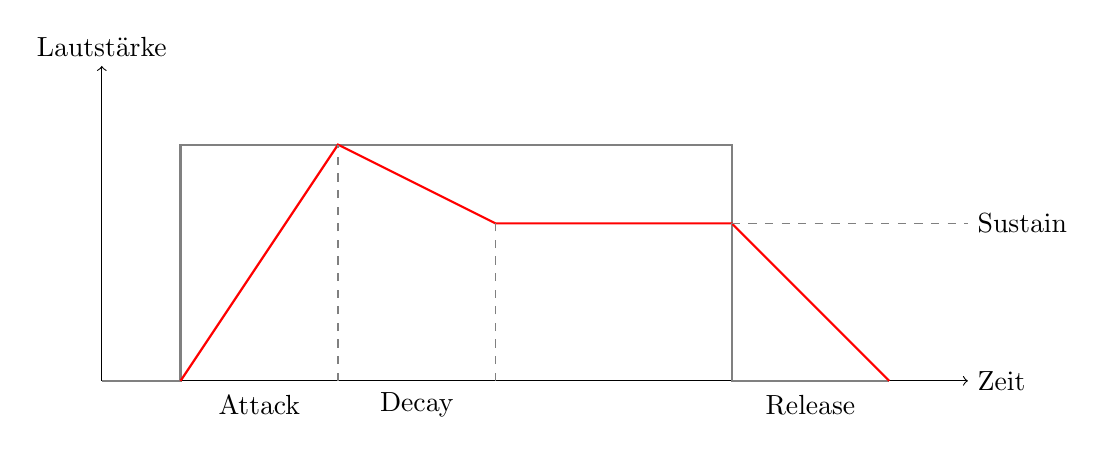
\begin{tikzpicture}
        % Achsen
        \draw[->] (0,0) -- (11,0) node[right] {Zeit};
        \draw[->] (0,0) -- (0,4) node[above] {Lautstärke};

        % Knopf gedrückt
        \draw[thick, gray] (0,0) -- (1,0) -- (1,3) -- (8,3) -- (8,0) -- (10,0);

        % Hüllkurve
        \draw[thick, red] (1,0) -- (3,3) -- (5,2) -- (8,2) -- (10,0);

        % Attack
        \draw[dashed, gray] (3,0) -- (3,3);
        \node at (2,-0.3) {Attack};

        % Decay
        \draw[dashed, gray] (5,0) -- (5,2);
        \node at (4,-0.3) {Decay};

        % Sustain
        \draw[dashed, gray] (8,2) -- (11,2) node[right, black] {Sustain};

        % Release
        \draw[dashed, gray] (8,0) -- (8,2);
        \node at (9,-0.3) {Release};

    \end{tikzpicture}
    \caption{Hüllkurve mit den 4 Parametern Attack, Decay, Sustain und Release}
    \label{fig:envelope}
\end{figure}

In Bild \ref{fig:envelope} sieht man in Grau wie der Knopf gedrückt und losgelassen 
wird und in Rot eine mögliche Hüllkurve.

\subsection{Vollständidiger Synthesizers}

Der Synthesizer so wie er zum Zeitpunkt der Abgabe dieser Arbeit implementiert ist, 
basiert auf dem einfachen Synthesizer aus Kapitel \ref{chap:simple_synth}. Zusätzlich wurde
eine Hüllkurve implementiert, welche die Lautstärke der einzelnen Töne
beeinflusst und es ist möglich folgende Parameter zu verändern:
\begin{itemize}
    \item Die Grundnote der Tonleiter
    \item Die Tonleiter
    \item Die WellenForm des Basses 
    \item Die Wellenform der einzelnen Töne
    \item Die Parameter der Hüllkurve
\end{itemize}

Welcher parameter gerade verändert wird, kann über ein Menü, welches auf dem Bildschirm
angezeigt wird, ausgewählt werden. Dieses Menü wird mit dem A und B Knopf und dem
Drehgeber bedient. Wie dies genau funktioniert wird in Kapitel \ref{chap:menu} erklärt.

Da die Generierung des Tons eine zeitkritische Aufgabe ist, darf sie nicht durch
das Lesen von Eingaben, das Schreiben auf den Bildschirm oder das Berechnen der
Hüllkurve unterbrochen werden. Deshalb wurden 3 freeRTOS-Tasks implementiert, 
welche die einzelnen Aufgaben übernehmen.

Um zwischen den Tasks zu kommunizieren, werden ThreadsaveVariables verwendet.
Das ist eine Klasse, welche nur eine Variable, einen Getter und einen Setter 
enthalten. Bei der Implementierung dieser Klassen wurde darauf geachteh, dass
die Getter und Setter Methoden Threadsafe sind. 

\subsubsection{Generierung des Tons}

Um einfach auf die Frequenzen der einzelnen Noten zugreifen zu können,
werden die Frequenzen in einem Array namens notes gespeichert. Die Grundnote einer
Tonleiter kann dann als Index g gespeichert und wenn die Tonleiter wie 
in Kapitel \ref{chap:music_theorie} beschrieben als Array names scale gespeichert ist,
kann auf Noten der Tonleiter wie folgt zugegriffen werden:
\begin{lstlisting}[language=C++,
                   frame=single,
                   caption={Zugriff auf die Frequenzen der Noten einer Tonleiter},
                   captionpos=b]
int noteFrequenzy = notes[g + scale[i]];
\end{lstlisting}

So lassen sich dei Grundnote und die Tonleiter einfach verändern.



\subsubsection{Berechnung der Hüllkurve}

\subsubsection{Menu}
\label{chap:menu}
TODO: Erklären wie das Menu funktioniert und wie es implementiert ist.